\section{Measurement}

In the present section, we will perform some measurements with the \gls{psd}.
In particular, we want to determine the spatial resolution and discuss the noise characteristics.

\subsection{Electrical setup}

\Cref{tab:equipment} lists the equipment required for the electrical setup.
The electric devices are connected as follows.
The \gls{psd} is connected with the power supply through the LEMO4 cable.
The DIFFX, DIFFY, and SUM output voltages of the \gls{psd} are conencted to the oscilloscope's first three input channels.
It is essential to use shielded cables to avoid receiving \SI{50}{\hertz} noise from surroudning switching power supplies.

\begin{table}[htb]
  \centering
  \begin{tabular}{ccl}
    \toprule
      Device & Amount \\
    \midrule
      \gls{psd} & 1\\
      Oscilloscope & 1\\
      \SI{\pm15}{\volt} voltage supply & 1\\
      Shielded LEMO4 cable & 1\\
      Shielded \acrshort{sma} cable & 3\\
      \acrshort{sma} to \acrshort{bnc} adapters & 3\\
    \bottomrule
  \end{tabular}
  \captionsetup{width=.8\textwidth}
  \caption{Electrical equipment required to operate the \gls{psd}}\label{tab:equipment}
\end{table}

You can configure the oscilloscope to show the first two input channels in X-Y mode.
In X-Y mode, the signal on the coordinate grid corresponds to the position of the incident light spot.
Suppose your light source shows strong intensity fluctuations.
In that case, you can use the oscilloscope's arithmetic operation to divide the DIFFX and DIFFY signals by the SUM signal.

\subsection{Optical setup}

\Cref{fig:optical_setup} shows an optical setup for spatial resolution measurements.
The arrangement comprises a laser source, two mirrors, a lens, and the \gls{psd}.
Using two mirrors instead of one allows more freedom in positioning the other optics.
The lens focuses the laser beam onto the sensitive area of the \gls{psd}.

\begin{figure}[htb]
	\centering
	\includestandalone[mode=buildnew]{figure/optic/setup}
	\caption{Optical setup for testing}\label{fig:optical_setup}
\end{figure}

\subsection{Grid scan}

\begin{figure}[htb]
	\centering
	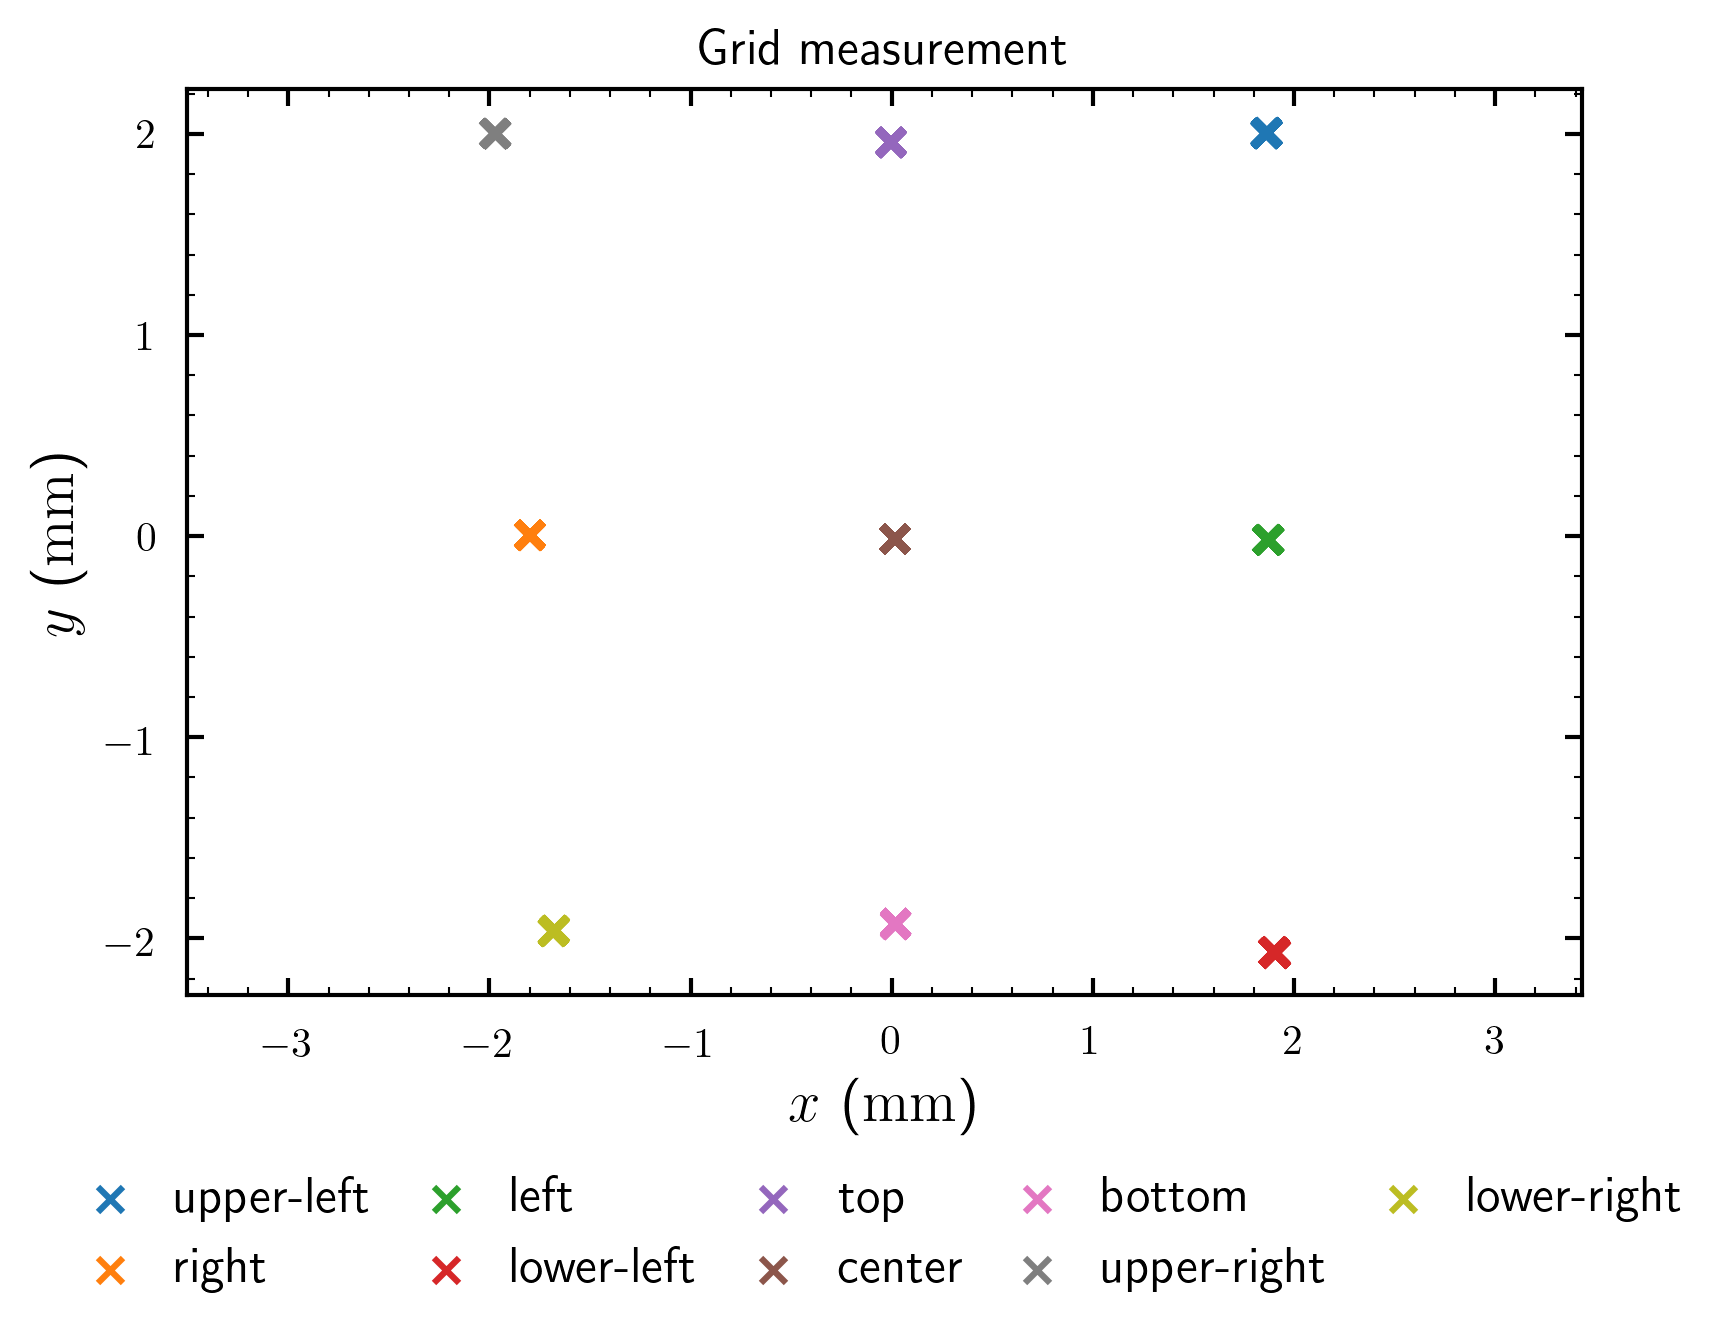
\includegraphics{figure/plot/grid-measurement}
	\caption{Spatial scan over $3\times 3$ grid by adjusting the mirrors.}\label{fig:grid_scan}
\end{figure}

\begin{figure}[htb]
	\centering
	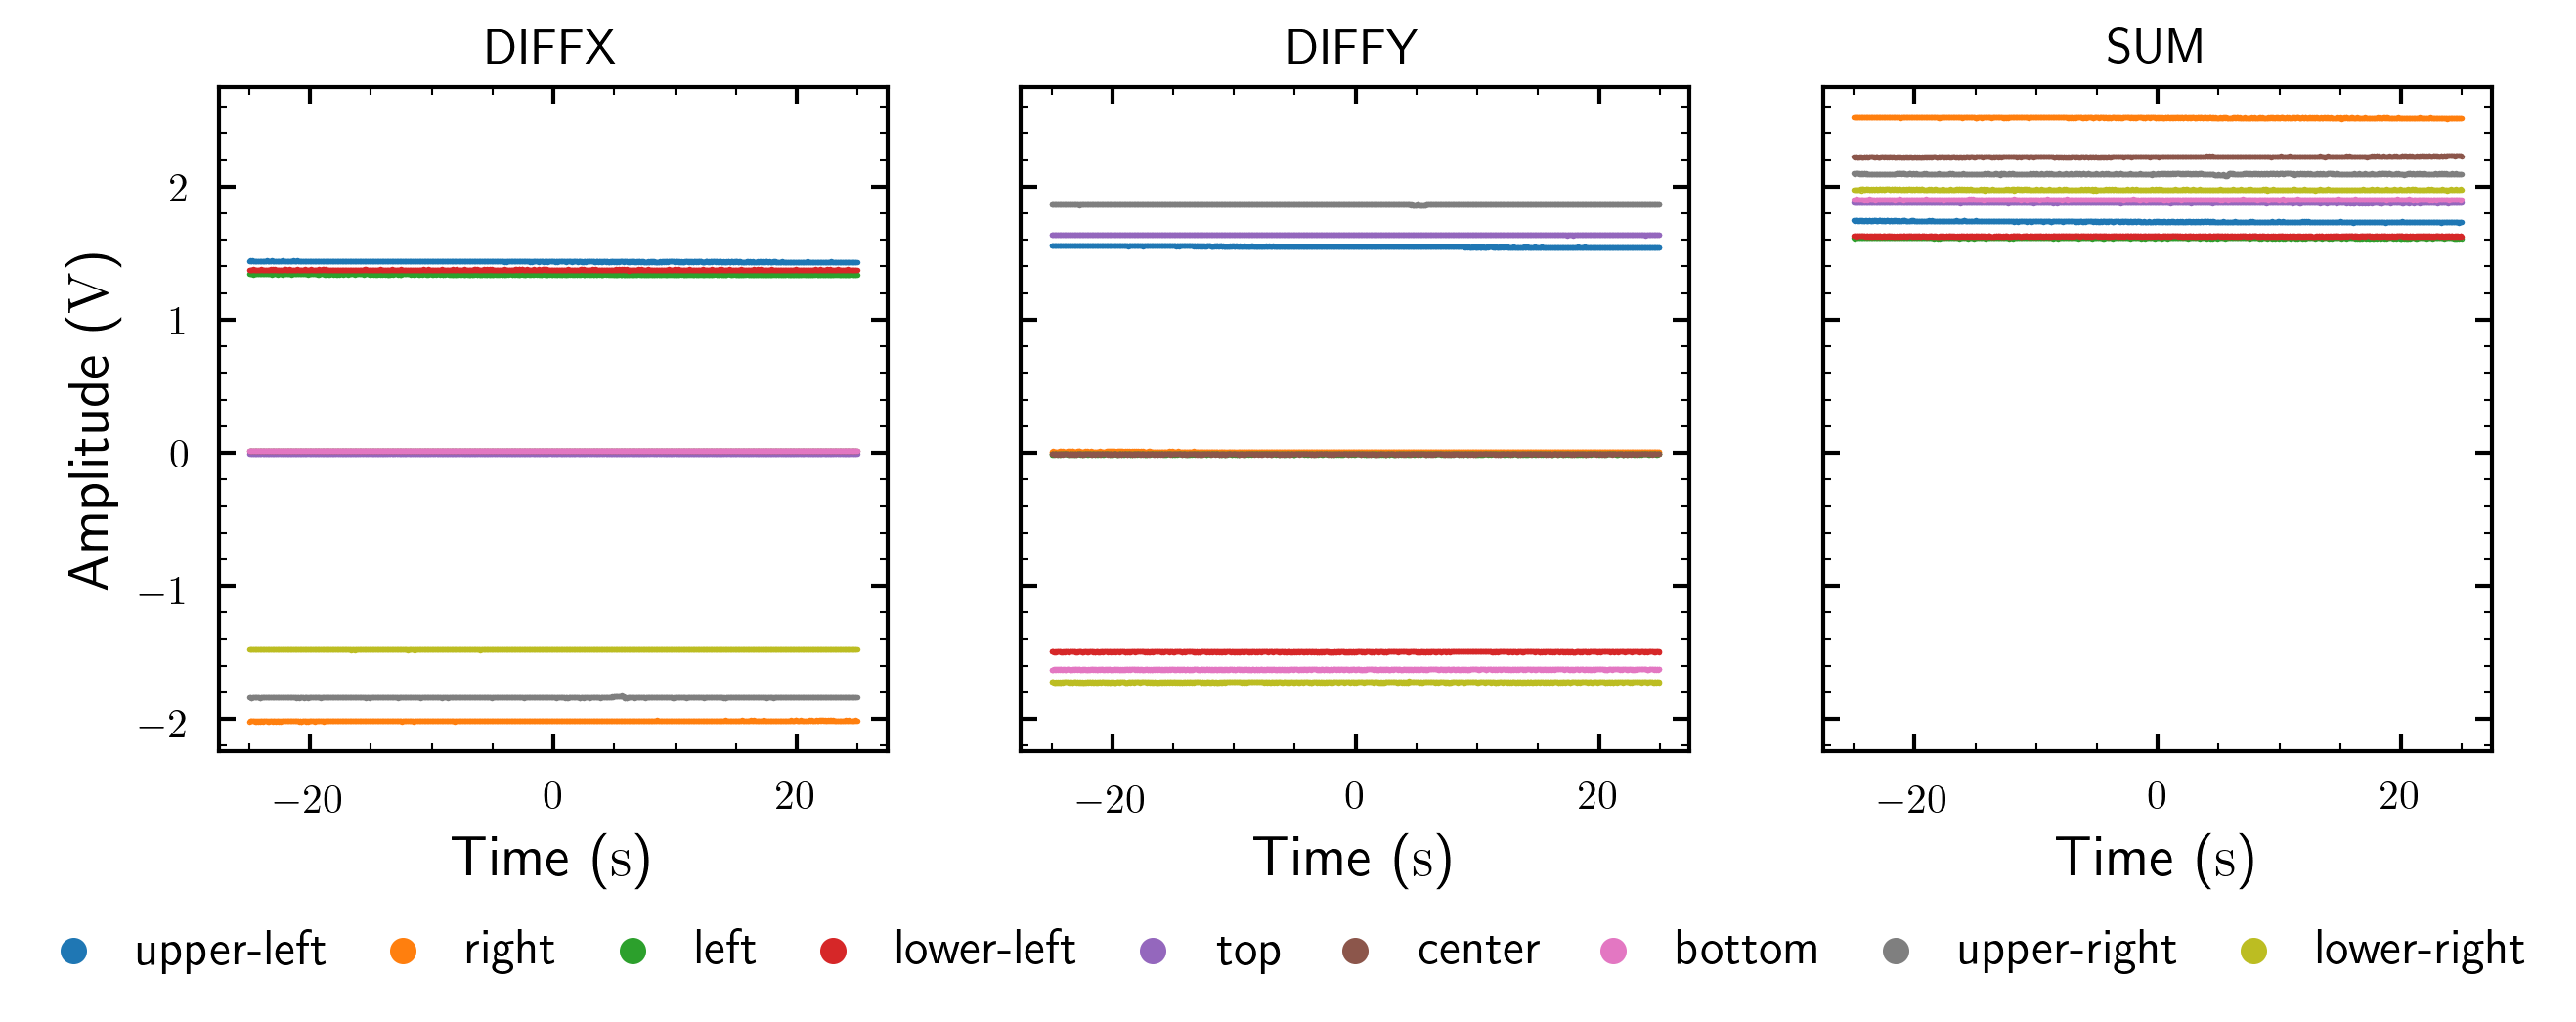
\includegraphics[scale=0.7]{figure/plot/voltages}
	\caption{Timeseries of the voltage signals captured during the grid scan.}\label{fig:grid_scan_voltages}
\end{figure}

\begin{align}
	\frac{(I_2+I_3)-(I_1+I_4)}{I_1+I_2+I_3+I_4}=\frac{2x}{L},
	&&
	\frac{(I_2+I_4)-(I_1+I_3)}{I_1+I_2+I_3+I_4}=\frac{2y}{L}
	\label{eq:position_conversion_photocurrent}
\end{align}
\begin{align}
	x=\frac{L}{2}\frac{\text{DIFFX}}{\text{SUM}}\ \si{\milli\meter}, &&
	y=\frac{L}{2}\frac{\text{DIFFY}}{\text{SUM}}\ \si{\milli\meter}.
	\label{eq:position_conversion_voltages}
\end{align}

\begin{figure}[htb]
	\centering
	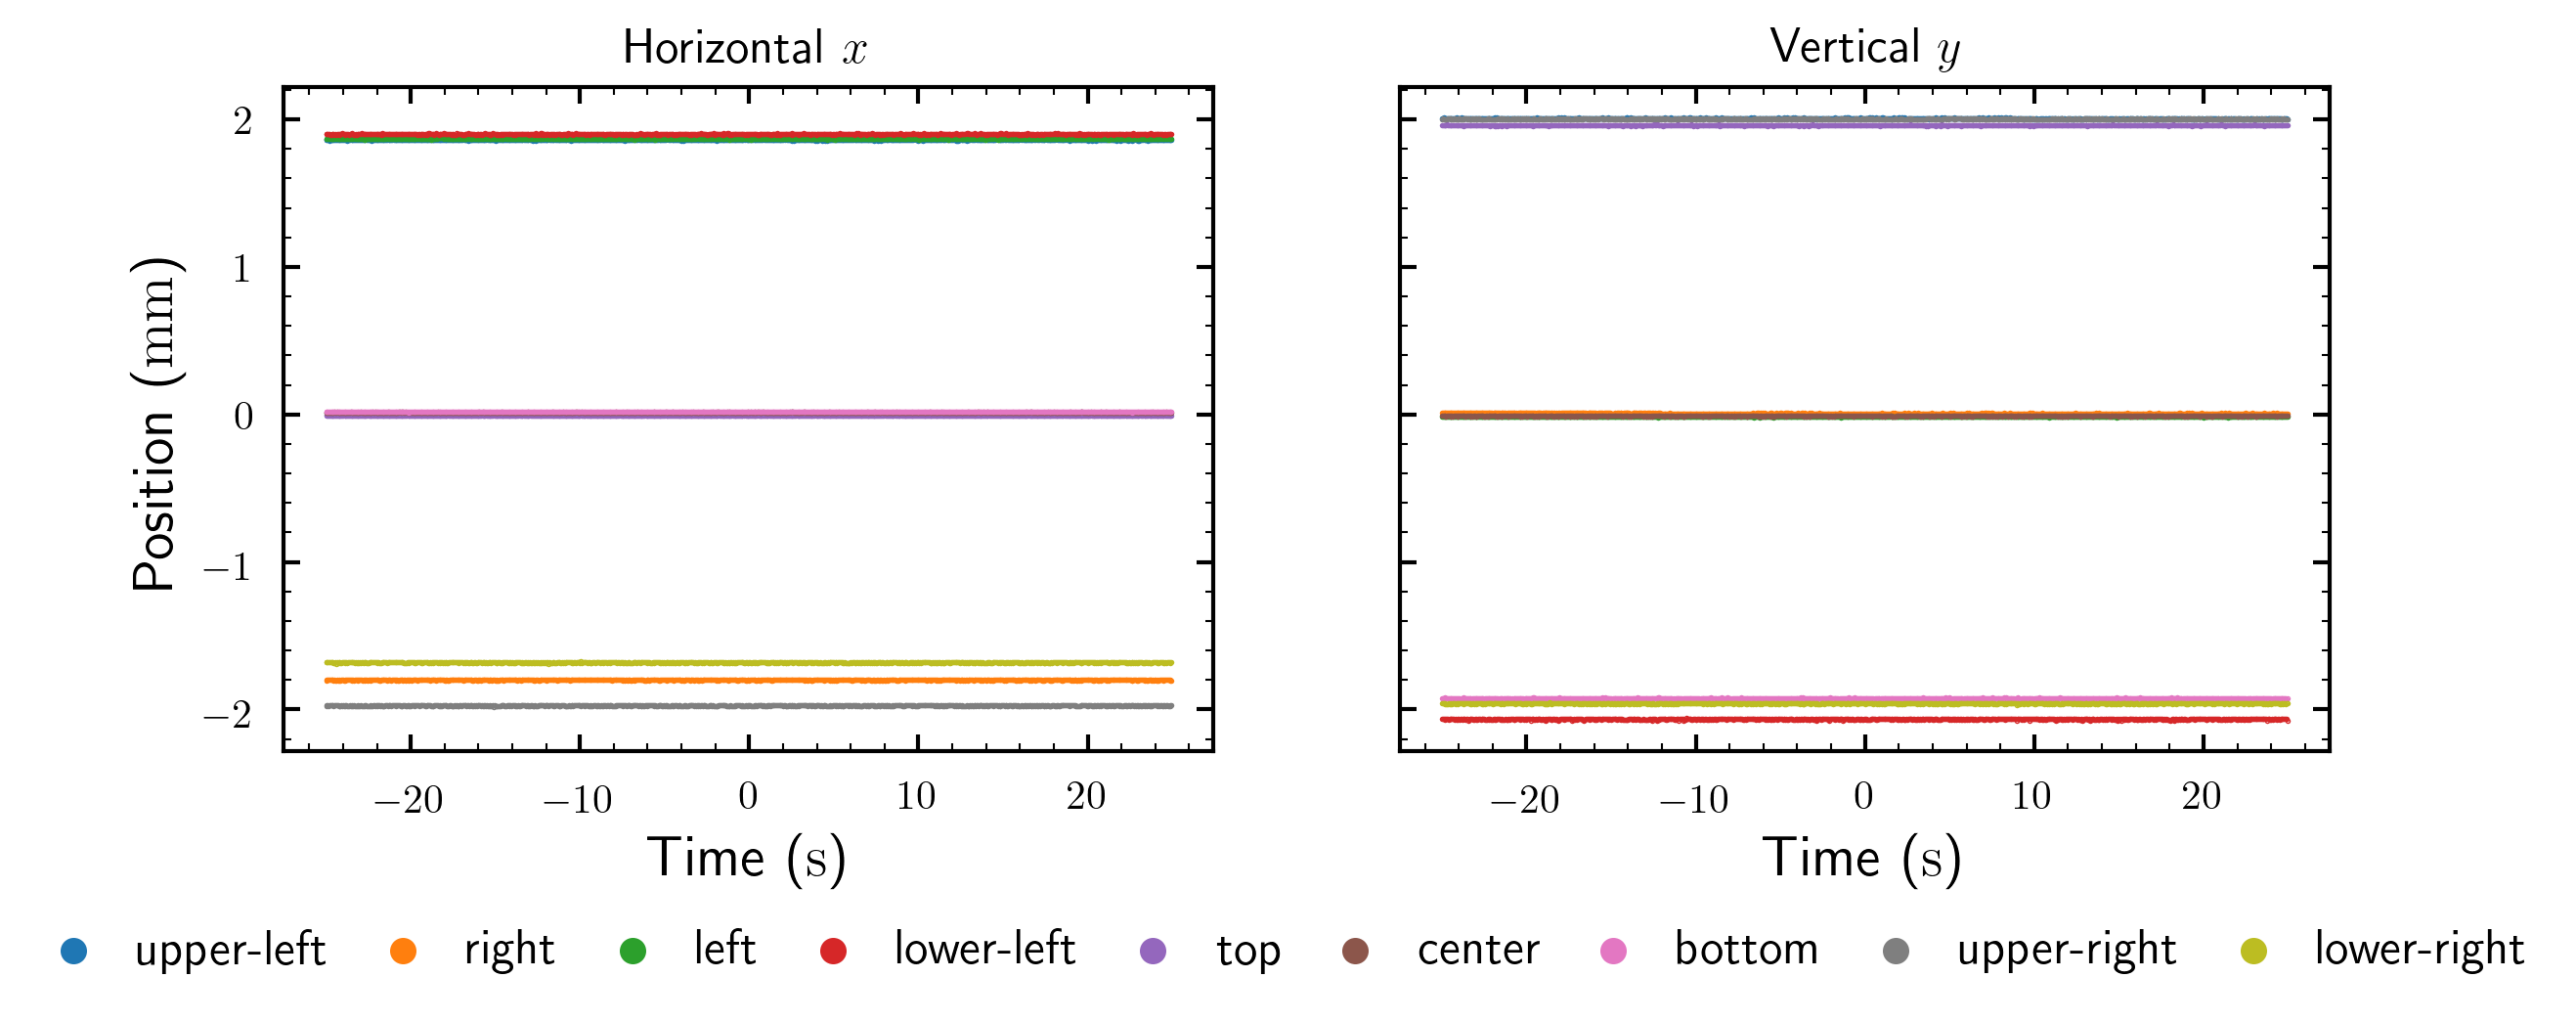
\includegraphics[scale=0.7]{figure/plot/positions}
	\caption{Voltage signals of the grid scan converted to positions.}\label{fig:grid_scan_x}
\end{figure}

% TODO: describe steps (oscilloscope settings, mirror adjustments)

\subsection{Resolution}

% TODO: estimate noise
% TODO: spatial resolution

\begin{table}[htb]
  \centering
  \begin{tabular}{lcccc}
    \toprule
      Measurement &
      $x$ (\si{\milli\meter}) &
      $\Delta x$ (\si{\milli\meter}) &
      $y$ (\si{\milli\meter}) &
      $\Delta y$ (\si{\milli\meter}) \\
    \midrule
      Center & \num{0.01} & \num{+1.08} & \num{-0.01} & \num{+1.03} \\      
      Top & \num{-0.01} & \num{+1.30} & \num{+1.96} & \num{+1.67} \\      
      Left & \num{1.87} & \num{+2.19} & \num{-0.01} & \num{+1.50} \\      
      Right & \num{-1.80} & \num{+1.38} & \num{+0.01} & \num{+1.61} \\
      Bottom & \num{0.02} & \num{+1.24} & \num{-1.92} & \num{+2.11} \\
      Upper left & \num{+1.86} & \num{+2.03} & \num{+2.01} & \num{+2.50} \\
      Upper right & \num{-1.97} & \num{+1.75} & \num{+2.00} & \num{+1.65} \\
      Lower left & \num{+1.90} & \num{+2.26} & \num{-2.07} & \num{+2.56} \\
      Lower right & \num{-1.68} & \num{+1.78} & \num{-1.96} & \num{+1.87} \\
    \bottomrule
  \end{tabular}
  \captionsetup{width=.8\textwidth}
  \caption{Position statistics of $3\times 3$ grid scan}\label{tab:grid_scan_position_statistics}
\end{table}

\begin{equation}
	z_R=\frac{\pi w_0^2}{\lambda}
	\label{eq:rayleigh_length}
\end{equation}

\begin{equation}
	w^\prime_0=\frac{w_0}{\sqrt{(1-s/f)^2+(z_R/f)^2}}
	\label{eq:beam_waist_thin_lens}
\end{equation}

\begin{table}[htb]
  \centering
  \begin{tabular}{lcc}
    \toprule
      Signal &
      Mean (\si{\milli\volt}) &
      Standard deviation (\si{\micro\meter}) \\
    \midrule
      DIFFX & \num{0.1} & \num{17} \\
      DIFFY & \num{0.4} & \num{17} \\
      SUM & \num{1.2} & \num{32} \\
    \bottomrule
  \end{tabular}
  \captionsetup{width=.8\textwidth}
  \caption{Signal statistics obtained without illumination}\label{tab:grid_scan_signal_statistics}
\end{table}

